\documentclass[tikz,border=2pt]{standalone}
\usepackage[T1]{fontenc}
\usepackage[scaled=0.95]{helvet}
\renewcommand{\familydefault}{\sfdefault}
\usetikzlibrary{arrows.meta}
% Chapter dependency map in the flat stack-diagram style (muted accent blocks, white
% bold type). Coordinates follow the original SVG; edges are unchanged from it.
\definecolor{accent}{HTML}{581C87}
\colorlet{stackfill}{accent!60!white}
\colorlet{bandfill}{accent!8!white}
\definecolor{ink}{RGB}{38,38,42}
\definecolor{softink}{RGB}{105,105,110}
\definecolor{lightlink}{RGB}{120,130,145}
\begin{document}
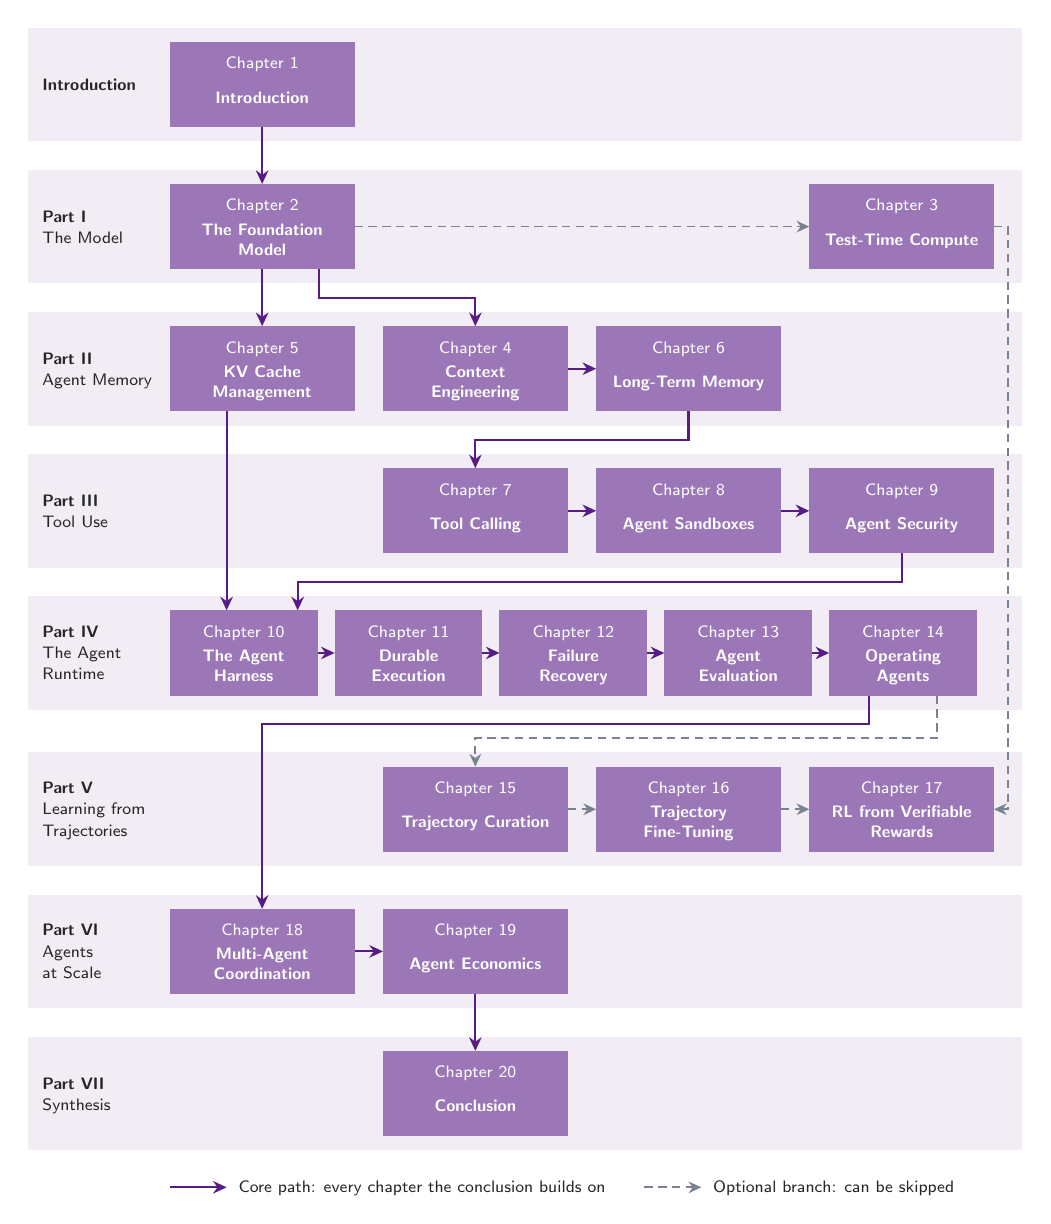
\begin{tikzpicture}[x=1pt,y=-1pt]

\fill[bandfill] (10.27,10.27) rectangle (369.73,51.35);
\fill[bandfill] (10.27,61.62) rectangle (369.73,102.70);
\fill[bandfill] (10.27,112.97) rectangle (369.73,154.05);
\fill[bandfill] (10.27,164.32) rectangle (369.73,205.41);
\fill[bandfill] (10.27,215.68) rectangle (369.73,256.76);
\fill[bandfill] (10.27,272.16) rectangle (369.73,313.24);
\fill[bandfill] (10.27,323.51) rectangle (369.73,364.59);
\fill[bandfill] (10.27,374.86) rectangle (369.73,415.95);
\fill[stackfill] (61.62,15.41) rectangle (128.38,46.22);
\fill[stackfill] (61.62,66.76) rectangle (128.38,97.57);
\fill[stackfill] (292.70,66.76) rectangle (359.46,97.57);
\fill[stackfill] (138.65,118.11) rectangle (205.41,148.92);
\fill[stackfill] (61.62,118.11) rectangle (128.38,148.92);
\fill[stackfill] (215.68,118.11) rectangle (282.43,148.92);
\fill[stackfill] (138.65,169.46) rectangle (205.41,200.27);
\fill[stackfill] (215.68,169.46) rectangle (282.43,200.27);
\fill[stackfill] (292.70,169.46) rectangle (359.46,200.27);
\fill[stackfill] (61.62,220.81) rectangle (115.03,251.62);
\fill[stackfill] (121.19,220.81) rectangle (174.59,251.62);
\fill[stackfill] (180.76,220.81) rectangle (234.16,251.62);
\fill[stackfill] (240.32,220.81) rectangle (293.73,251.62);
\fill[stackfill] (299.89,220.81) rectangle (353.30,251.62);
\fill[stackfill] (138.65,277.30) rectangle (205.41,308.11);
\fill[stackfill] (215.68,277.30) rectangle (282.43,308.11);
\fill[stackfill] (292.70,277.30) rectangle (359.46,308.11);
\fill[stackfill] (61.62,328.65) rectangle (128.38,359.46);
\fill[stackfill] (138.65,328.65) rectangle (205.41,359.46);
\fill[stackfill] (138.65,380.00) rectangle (205.41,410.81);
\node[anchor=base west,inner sep=0pt,text=ink,font=\bfseries\fontsize{6.2}{7.1}\selectfont] at (15.41,32.86) {Introduction};
\node[anchor=base west,inner sep=0pt,text=ink,font=\bfseries\fontsize{6.2}{7.1}\selectfont] at (15.41,80.62) {Part I};
\node[anchor=base west,inner sep=0pt,text=ink,font=\fontsize{5.9}{6.8}\selectfont] at (15.41,88.32) {The Model};
\node[anchor=base west,inner sep=0pt,text=ink,font=\bfseries\fontsize{6.2}{7.1}\selectfont] at (15.41,131.97) {Part II};
\node[anchor=base west,inner sep=0pt,text=ink,font=\fontsize{5.9}{6.8}\selectfont] at (15.41,139.68) {Agent Memory};
\node[anchor=base west,inner sep=0pt,text=ink,font=\bfseries\fontsize{6.2}{7.1}\selectfont] at (15.41,183.32) {Part III};
\node[anchor=base west,inner sep=0pt,text=ink,font=\fontsize{5.9}{6.8}\selectfont] at (15.41,191.03) {Tool Use};
\node[anchor=base west,inner sep=0pt,text=ink,font=\bfseries\fontsize{6.2}{7.1}\selectfont] at (15.41,230.57) {Part IV};
\node[anchor=base west,inner sep=0pt,text=ink,font=\fontsize{5.9}{6.8}\selectfont] at (15.41,238.27) {The Agent};
\node[anchor=base west,inner sep=0pt,text=ink,font=\fontsize{5.9}{6.8}\selectfont] at (15.41,245.97) {Runtime};
\node[anchor=base west,inner sep=0pt,text=ink,font=\bfseries\fontsize{6.2}{7.1}\selectfont] at (15.41,287.05) {Part V};
\node[anchor=base west,inner sep=0pt,text=ink,font=\fontsize{5.9}{6.8}\selectfont] at (15.41,294.76) {Learning from};
\node[anchor=base west,inner sep=0pt,text=ink,font=\fontsize{5.9}{6.8}\selectfont] at (15.41,302.46) {Trajectories};
\node[anchor=base west,inner sep=0pt,text=ink,font=\bfseries\fontsize{6.2}{7.1}\selectfont] at (15.41,338.41) {Part VI};
\node[anchor=base west,inner sep=0pt,text=ink,font=\fontsize{5.9}{6.8}\selectfont] at (15.41,346.11) {Agents};
\node[anchor=base west,inner sep=0pt,text=ink,font=\fontsize{5.9}{6.8}\selectfont] at (15.41,353.81) {at Scale};
\node[anchor=base west,inner sep=0pt,text=ink,font=\bfseries\fontsize{6.2}{7.1}\selectfont] at (15.41,393.86) {Part VII};
\node[anchor=base west,inner sep=0pt,text=ink,font=\fontsize{5.9}{6.8}\selectfont] at (15.41,401.57) {Synthesis};
\node[anchor=base,inner sep=0pt,text=white,font=\fontsize{5.9}{6.8}\selectfont] at (95.00,25.16) {Chapter 1};
\node[anchor=base,inner sep=0pt,text=white,font=\bfseries\fontsize{6.2}{7.1}\selectfont] at (95.00,37.49) {Introduction};
\node[anchor=base,inner sep=0pt,text=white,font=\fontsize{5.9}{6.8}\selectfont] at (95.00,76.51) {Chapter 2};
\node[anchor=base,inner sep=0pt,text=white,font=\bfseries\fontsize{6.2}{7.1}\selectfont] at (95.00,85.24) {The Foundation};
\node[anchor=base,inner sep=0pt,text=white,font=\bfseries\fontsize{6.2}{7.1}\selectfont] at (95.00,92.43) {Model};
\node[anchor=base,inner sep=0pt,text=white,font=\fontsize{5.9}{6.8}\selectfont] at (326.08,76.51) {Chapter 3};
\node[anchor=base,inner sep=0pt,text=white,font=\bfseries\fontsize{6.2}{7.1}\selectfont] at (326.08,88.84) {Test-Time Compute};
\node[anchor=base,inner sep=0pt,text=white,font=\fontsize{5.9}{6.8}\selectfont] at (172.03,127.86) {Chapter 4};
\node[anchor=base,inner sep=0pt,text=white,font=\bfseries\fontsize{6.2}{7.1}\selectfont] at (172.03,136.59) {Context};
\node[anchor=base,inner sep=0pt,text=white,font=\bfseries\fontsize{6.2}{7.1}\selectfont] at (172.03,143.78) {Engineering};
\node[anchor=base,inner sep=0pt,text=white,font=\fontsize{5.9}{6.8}\selectfont] at (95.00,127.86) {Chapter 5};
\node[anchor=base,inner sep=0pt,text=white,font=\bfseries\fontsize{6.2}{7.1}\selectfont] at (95.00,136.59) {KV Cache};
\node[anchor=base,inner sep=0pt,text=white,font=\bfseries\fontsize{6.2}{7.1}\selectfont] at (95.00,143.78) {Management};
\node[anchor=base,inner sep=0pt,text=white,font=\fontsize{5.9}{6.8}\selectfont] at (249.05,127.86) {Chapter 6};
\node[anchor=base,inner sep=0pt,text=white,font=\bfseries\fontsize{6.2}{7.1}\selectfont] at (249.05,140.19) {Long-Term Memory};
\node[anchor=base,inner sep=0pt,text=white,font=\fontsize{5.9}{6.8}\selectfont] at (172.03,179.22) {Chapter 7};
\node[anchor=base,inner sep=0pt,text=white,font=\bfseries\fontsize{6.2}{7.1}\selectfont] at (172.03,191.54) {Tool Calling};
\node[anchor=base,inner sep=0pt,text=white,font=\fontsize{5.9}{6.8}\selectfont] at (249.05,179.22) {Chapter 8};
\node[anchor=base,inner sep=0pt,text=white,font=\bfseries\fontsize{6.2}{7.1}\selectfont] at (249.05,191.54) {Agent Sandboxes};
\node[anchor=base,inner sep=0pt,text=white,font=\fontsize{5.9}{6.8}\selectfont] at (326.08,179.22) {Chapter 9};
\node[anchor=base,inner sep=0pt,text=white,font=\bfseries\fontsize{6.2}{7.1}\selectfont] at (326.08,191.54) {Agent Security};
\node[anchor=base,inner sep=0pt,text=white,font=\fontsize{5.9}{6.8}\selectfont] at (88.32,230.57) {Chapter 10};
\node[anchor=base,inner sep=0pt,text=white,font=\bfseries\fontsize{6.2}{7.1}\selectfont] at (88.32,239.30) {The Agent};
\node[anchor=base,inner sep=0pt,text=white,font=\bfseries\fontsize{6.2}{7.1}\selectfont] at (88.32,246.49) {Harness};
\node[anchor=base,inner sep=0pt,text=white,font=\fontsize{5.9}{6.8}\selectfont] at (147.89,230.57) {Chapter 11};
\node[anchor=base,inner sep=0pt,text=white,font=\bfseries\fontsize{6.2}{7.1}\selectfont] at (147.89,239.30) {Durable};
\node[anchor=base,inner sep=0pt,text=white,font=\bfseries\fontsize{6.2}{7.1}\selectfont] at (147.89,246.49) {Execution};
\node[anchor=base,inner sep=0pt,text=white,font=\fontsize{5.9}{6.8}\selectfont] at (207.46,230.57) {Chapter 12};
\node[anchor=base,inner sep=0pt,text=white,font=\bfseries\fontsize{6.2}{7.1}\selectfont] at (207.46,239.30) {Failure};
\node[anchor=base,inner sep=0pt,text=white,font=\bfseries\fontsize{6.2}{7.1}\selectfont] at (207.46,246.49) {Recovery};
\node[anchor=base,inner sep=0pt,text=white,font=\fontsize{5.9}{6.8}\selectfont] at (267.03,230.57) {Chapter 13};
\node[anchor=base,inner sep=0pt,text=white,font=\bfseries\fontsize{6.2}{7.1}\selectfont] at (267.03,239.30) {Agent};
\node[anchor=base,inner sep=0pt,text=white,font=\bfseries\fontsize{6.2}{7.1}\selectfont] at (267.03,246.49) {Evaluation};
\node[anchor=base,inner sep=0pt,text=white,font=\fontsize{5.9}{6.8}\selectfont] at (326.59,230.57) {Chapter 14};
\node[anchor=base,inner sep=0pt,text=white,font=\bfseries\fontsize{6.2}{7.1}\selectfont] at (326.59,239.30) {Operating};
\node[anchor=base,inner sep=0pt,text=white,font=\bfseries\fontsize{6.2}{7.1}\selectfont] at (326.59,246.49) {Agents};
\node[anchor=base,inner sep=0pt,text=white,font=\fontsize{5.9}{6.8}\selectfont] at (172.03,287.05) {Chapter 15};
\node[anchor=base,inner sep=0pt,text=white,font=\bfseries\fontsize{6.2}{7.1}\selectfont] at (172.03,299.38) {Trajectory Curation};
\node[anchor=base,inner sep=0pt,text=white,font=\fontsize{5.9}{6.8}\selectfont] at (249.05,287.05) {Chapter 16};
\node[anchor=base,inner sep=0pt,text=white,font=\bfseries\fontsize{6.2}{7.1}\selectfont] at (249.05,295.78) {Trajectory};
\node[anchor=base,inner sep=0pt,text=white,font=\bfseries\fontsize{6.2}{7.1}\selectfont] at (249.05,302.97) {Fine-Tuning};
\node[anchor=base,inner sep=0pt,text=white,font=\fontsize{5.9}{6.8}\selectfont] at (326.08,287.05) {Chapter 17};
\node[anchor=base,inner sep=0pt,text=white,font=\bfseries\fontsize{6.2}{7.1}\selectfont] at (326.08,295.78) {RL from Verifiable};
\node[anchor=base,inner sep=0pt,text=white,font=\bfseries\fontsize{6.2}{7.1}\selectfont] at (326.08,302.97) {Rewards};
\node[anchor=base,inner sep=0pt,text=white,font=\fontsize{5.9}{6.8}\selectfont] at (95.00,338.41) {Chapter 18};
\node[anchor=base,inner sep=0pt,text=white,font=\bfseries\fontsize{6.2}{7.1}\selectfont] at (95.00,347.14) {Multi-Agent};
\node[anchor=base,inner sep=0pt,text=white,font=\bfseries\fontsize{6.2}{7.1}\selectfont] at (95.00,354.32) {Coordination};
\node[anchor=base,inner sep=0pt,text=white,font=\fontsize{5.9}{6.8}\selectfont] at (172.03,338.41) {Chapter 19};
\node[anchor=base,inner sep=0pt,text=white,font=\bfseries\fontsize{6.2}{7.1}\selectfont] at (172.03,350.73) {Agent Economics};
\node[anchor=base,inner sep=0pt,text=white,font=\fontsize{5.9}{6.8}\selectfont] at (172.03,389.76) {Chapter 20};
\node[anchor=base,inner sep=0pt,text=white,font=\bfseries\fontsize{6.2}{7.1}\selectfont] at (172.03,402.08) {Conclusion};
\node[anchor=base west,inner sep=0pt,text=ink,font=\fontsize{5.9}{6.8}\selectfont] at (86.27,431.35) {Core path: every chapter the conclusion builds on};
\node[anchor=base west,inner sep=0pt,text=ink,font=\fontsize{5.9}{6.8}\selectfont] at (257.78,431.35) {Optional branch: can be skipped};
\draw[accent,line width=0.77pt,-{Stealth[length=4.9pt,width=4.5pt]}] (95.00,46.22) -- (95.00,66.76);
\draw[accent,line width=0.77pt,-{Stealth[length=4.9pt,width=4.5pt]}] (95.00,97.57) -- (95.00,118.11);
\draw[accent,line width=0.77pt,-{Stealth[length=4.9pt,width=4.5pt]}] (115.54,97.57) -- (115.54,107.84) -- (172.03,107.84) -- (172.03,118.11);
\draw[lightlink,line width=0.62pt,dash pattern=on 3pt off 2pt,-{Stealth[length=4.6pt,width=4.2pt]}] (128.38,82.16) -- (292.70,82.16);
\draw[accent,line width=0.77pt,-{Stealth[length=4.9pt,width=4.5pt]}] (205.41,133.51) -- (215.68,133.51);
\draw[accent,line width=0.77pt,-{Stealth[length=4.9pt,width=4.5pt]}] (249.05,148.92) -- (249.05,159.19) -- (172.03,159.19) -- (172.03,169.46);
\draw[accent,line width=0.77pt,-{Stealth[length=4.9pt,width=4.5pt]}] (205.41,184.86) -- (215.68,184.86);
\draw[accent,line width=0.77pt,-{Stealth[length=4.9pt,width=4.5pt]}] (282.43,184.86) -- (292.70,184.86);
\draw[accent,line width=0.77pt,-{Stealth[length=4.9pt,width=4.5pt]}] (82.16,148.92) -- (82.16,220.81);
\draw[accent,line width=0.77pt,-{Stealth[length=4.9pt,width=4.5pt]}] (326.08,200.27) -- (326.08,210.54) -- (107.84,210.54) -- (107.84,220.81);
\draw[accent,line width=0.77pt,-{Stealth[length=4.9pt,width=4.5pt]}] (115.03,236.22) -- (121.19,236.22);
\draw[accent,line width=0.77pt,-{Stealth[length=4.9pt,width=4.5pt]}] (174.59,236.22) -- (180.76,236.22);
\draw[accent,line width=0.77pt,-{Stealth[length=4.9pt,width=4.5pt]}] (234.16,236.22) -- (240.32,236.22);
\draw[accent,line width=0.77pt,-{Stealth[length=4.9pt,width=4.5pt]}] (293.73,236.22) -- (299.89,236.22);
\draw[accent,line width=0.77pt,-{Stealth[length=4.9pt,width=4.5pt]}] (128.38,344.05) -- (138.65,344.05);
\draw[accent,line width=0.77pt,-{Stealth[length=4.9pt,width=4.5pt]}] (314.27,251.62) -- (314.27,261.89) -- (95.00,261.89) -- (95.00,328.65);
\draw[lightlink,line width=0.62pt,dash pattern=on 3pt off 2pt,-{Stealth[length=4.6pt,width=4.2pt]}] (338.92,251.62) -- (338.92,267.03) -- (172.03,267.03) -- (172.03,277.30);
\draw[lightlink,line width=0.62pt,dash pattern=on 3pt off 2pt,-{Stealth[length=4.6pt,width=4.2pt]}] (205.41,292.70) -- (215.68,292.70);
\draw[lightlink,line width=0.62pt,dash pattern=on 3pt off 2pt,-{Stealth[length=4.6pt,width=4.2pt]}] (282.43,292.70) -- (292.70,292.70);
\draw[lightlink,line width=0.62pt,dash pattern=on 3pt off 2pt,-{Stealth[length=4.6pt,width=4.2pt]}] (359.46,82.16) -- (364.59,82.16) -- (364.59,292.70) -- (359.46,292.70);
\draw[accent,line width=0.77pt,-{Stealth[length=4.9pt,width=4.5pt]}] (172.03,359.46) -- (172.03,380.00);
\draw[accent,line width=0.77pt,-{Stealth[length=4.9pt,width=4.5pt]}] (61.62,429.30) -- (82.16,429.30);
\draw[lightlink,line width=0.62pt,dash pattern=on 3pt off 2pt,-{Stealth[length=4.6pt,width=4.2pt]}] (233.14,429.30) -- (253.68,429.30);
\end{tikzpicture}
\end{document}
